\documentclass{beamer}
% Die Hyperref Option hyperref={pdfpagelabels=false} verhindert die Warnung:
% Package hyperref Warning: Option `pdfpagelabels' is turned off
% (hyperref)                because \thepage is undefined. 
% Hyperref stopped early 
%
\usepackage{amsmath}
\usepackage{float}
\usepackage{lmodern}
\usepackage[font=footnotesize]{caption}
% Das Paket lmodern erspart die folgenden Warnungen:
% LaTeX Font Warning: Font shape `OT1/cmss/m/n' in size <4> not available
% (Font)              size <5> substituted on input line 22.
% LaTeX Font Warning: Size substitutions with differences
% (Font)              up to 1.0pt have occurred.
%

% Wenn \titel{\ldots} \author{\ldots} erst nach \begin{document} kommen,
% kommt folgende Warnung:
% Package hyperref Warning: Option `pdfauthor' has already been used,
% (hyperref) ... 
% Daher steht es hier vor \begin{document}

\title{\textbf{Quality Control Tool: Adaption to raw data}}
\subtitle{IDP im Sommersemester 2013}  
\author{Sarah Barton und Sonja Vogl} 
\date{4.7.2013} 

% Dadurch wird verhindert, dass die Navigationsleiste angezeigt wird.
\setbeamertemplate{navigation symbols}{}

% zusaetzlich ist das usepackage{beamerthemeshadow} eingebunden 
\usepackage{beamerthemeshadow}

%  \beamersetuncovermixins{\opaqueness<1>{25}}{\opaqueness<2->{15}}
%  sorgt dafuer das die Elemente die erst noch (zukuenftig) kommen 
%  nur schwach angedeutet erscheinen 
\beamersetuncovermixins{\opaqueness<1>{25}}{\opaqueness<2->{15}}
% klappt auch bei Tabellen, wenn teTeX verwendet wird\ldots
\begin{document}


\begin{frame}
\titlepage
\end{frame} 

\begin{frame}
\frametitle{Inhaltsverzeichnis}
\tableofcontents
\end{frame} 


\section{GUI des QualityControlTools} 
\begin{frame}
\frametitle{GUI des QualityControlTools } 
\begin{figure}[H]
\centerline{
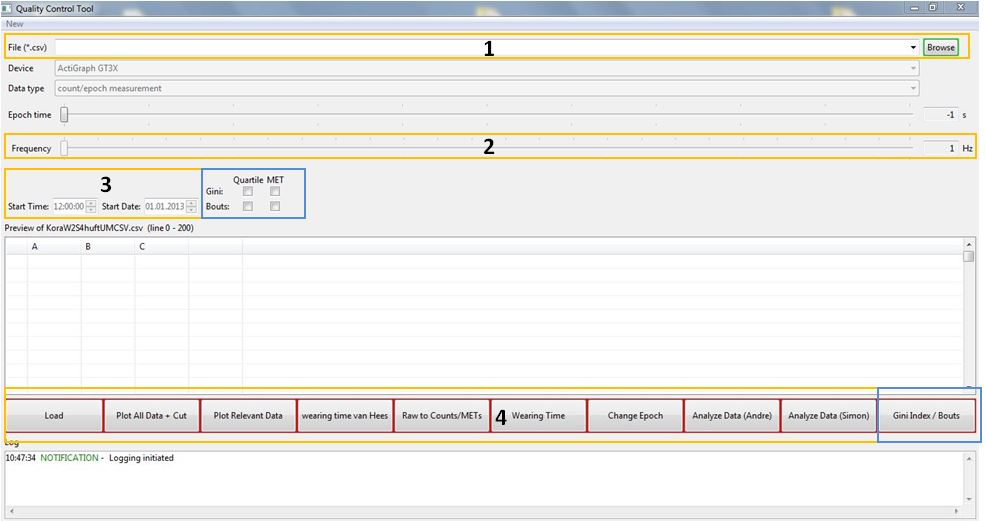
\includegraphics[width=100mm, height=50mm]{Abbildungen/ErweitertesTool1.JPG}
}
\caption {GUI des QualityControlTools 2. Version}
\end{figure}

\end{frame}

\end{document}
